\iffalse
\documentclass[10pt, a4paper]{article}
\usepackage[a4paper,outer=1.5cm,inner=1.5cm,top=1.75cm,bottom=1.5cm]{geometry}

\twocolumn
\usepackage{graphicx}

\usepackage{hyperref}
\usepackage[utf8]{inputenc}
\usepackage{amsmath}
\usepackage{physics}
\usepackage{amssymb}
\begin{document}
\title{Assignment-4}
\author{Name:C.CHANDANA\and Email :  \url{cheenepallichandana531@gmail.com}}
%\{ Wireless Communication (FWC)}
\date{30-sep-2022}
\maketitle



\section{Problem}
\fi
If three points $(x, -1), (2, 1)$ and $(4, 5)$ are collinear, find the value of $x$.
\\
\solution 
	\begin{figure}[!ht]
		\centering
 \includegraphics[width=\columnwidth]{chapters/11/10/1/8/figs/sline.png}
		\caption{}
		\label{fig:11/10/1/8}
  	\end{figure}
	\iffalse
\begin{center}
	\fi
	Let
\begin{align} \label{eq:11/10/1/8}
	\vec{A}=\myvec{ x\\ -1 },
	\vec{B}=\myvec{ 2\\ 1 },
\vec{C}=\myvec{ 4\\ 5 }.
\end{align}
Then
\begin{align}
\vec{A}-\vec{B}
	&=\myvec{ x-2\\ -2 }
	\\
\vec{A}-\vec{C}
	&=\myvec{ 4-x\\ 6 }
\end{align}
Forming the collinearity matrix
using 
	\eqref{eq:normal_line-collinear},
\begin{align} 
\myvec{ x-2 & -2\\ 4-x & 6  } 
	\xleftrightarrow[]{{R_1=3R_1+R-2}}
=\myvec{
2x-2 &0 \\ 
 4-x& 6
}
\end{align}

\iffalse

In the problem they have given that three points lie on a line, thats means these three points are collinear.\\

If  points on a line  are  collinear, rank of matrix is " 1 "then the vectors are in linearlydependent.\\
For 2 × 2 matrix Rank =1 means Determinant is 0.\\

Through pivoting,we obtain\\
\begin{align}
=\myvec{ x-2 & -2\\ 4-x & 6 \ } \\ 
\end{align}
\begin{align}
=\myvec{
x-2 &-2 \\ 
 4-x& 6
}\overset{R1=3R1+R2}{\rightarrow}
=\myvec{
2x-2 &0 \\ 
 4-x& 6
}
\end{align} 
\fi
	If the rank of the matrix is 1, any one of the rows must be zero. So, making the first element in the above matrix 0,
\begin{align}
x=1
\end{align} 

\iffalse

\begin{align}\label{eq:11/10/1/8}
x=1 \\
\end{align} 

Hence proved.\\
\section{Construction}
 \begin{figure}[h]
\centering
\includegraphics[scale=0.4]{sline.png} 
\caption{}
\end{figure}
\section{Code}
*Verify the above proofs in the following code.\\
\framebox{
\url{https://github.com/chandana531/FWC/tree/main/matrix/line}}	
\bibliographystyle{ieeetr}
\end{document}
\fi
